\chapter{Drupal Views}

\section{User management}

Before digging into the Drupal Views module we are going to learn some things about user management. Out of the box Drupal provides powerful user management features. We can create users with different roles. A role defines a set of permissions. For example: a \textbf{moderator} role could have the permissions \textbf{Administer comment types and settings} and \textbf{Administer comments and comment settings}. To manage the user settings go to the \textbf{People} tab in the management menu (Figure \ref{fig:people_menu}).

  \begin{figure}[H]
  	\centering
  	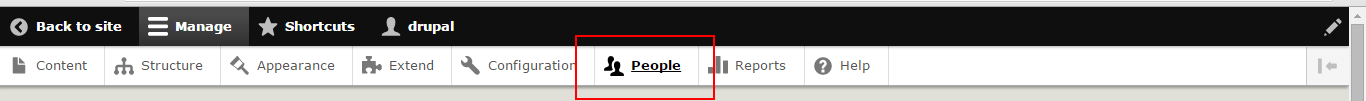
\includegraphics[width=\textwidth]{chapter6/people_menu}
  	\label{fig:people_menu}
  \end{figure}
  
  The \textbf{People} page has three tabs: \textbf{List}, \textbf{Permissions} and \textbf{Roles} (Figure \ref{fig:people_page}).
  
   \begin{figure}[H]
   	\centering
   	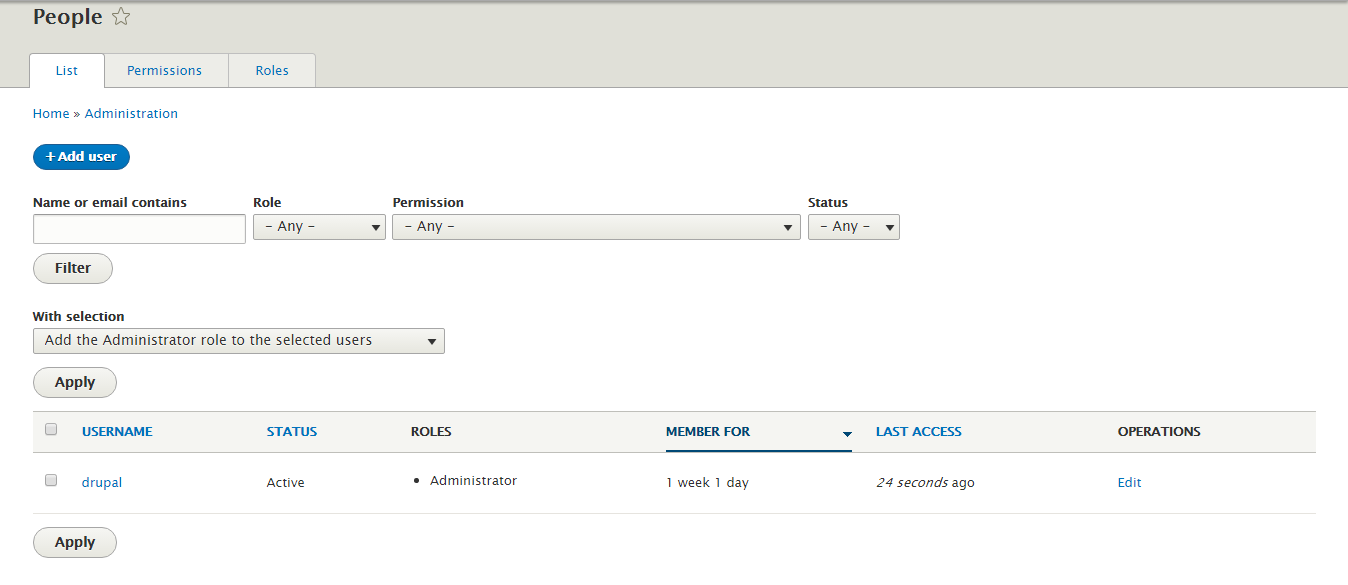
\includegraphics[width=\textwidth]{chapter6/people_page}
   	\label{fig:people_page}
   \end{figure}  
   
   These three pages define the following functionality:
   
   \begin{description}
   	 \item[List] Shows a list of all users, allows you to search trough the users and edit them.
   	 \item[Permissions] This page lists all the site permissions vertically and user roles horizontally. For each role you can select its permissions by checking the check-boxes (\ref{fig:permissions_page}). 
   	 
   	 \begin{figure}[H]
   	 	\centering
   	 	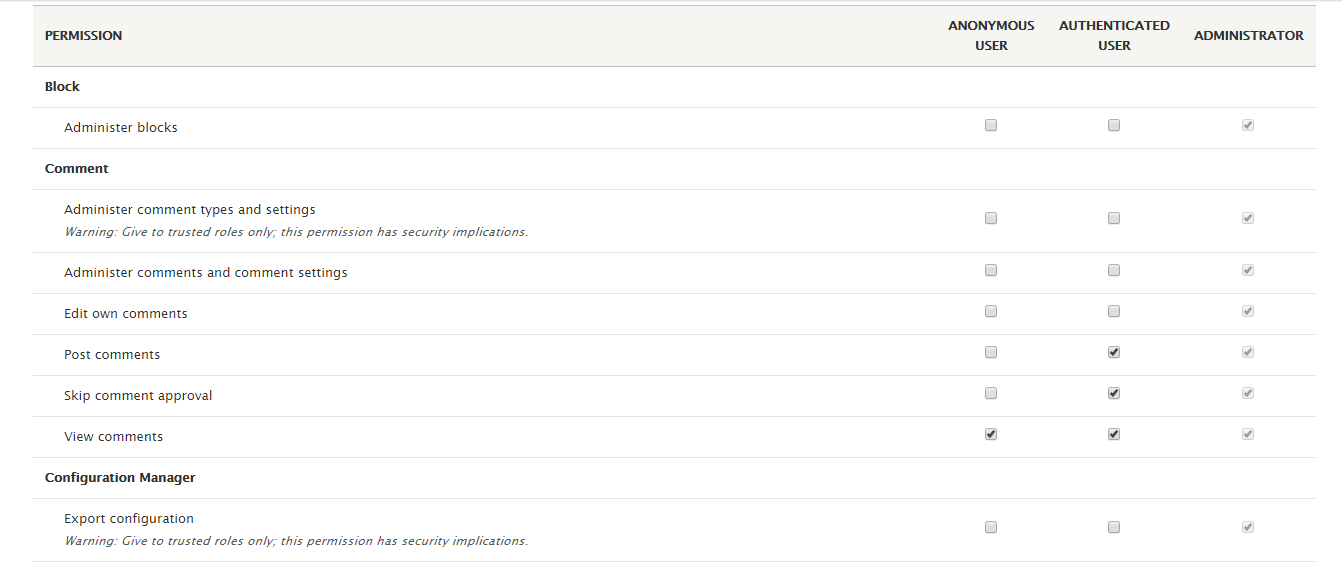
\includegraphics[width=\textwidth]{chapter6/permissions_page}
   	 	\caption{Permissions page.}
   	 	\label{fig:permissions_page}
   	 \end{figure}
   	 
   	 \item[Roles] This page allows you to add, remove and edit roles. When you add a new role, it will appear on the permissions page.
   	 
   	 \begin{figure}[H]
   	 	\centering
   	 	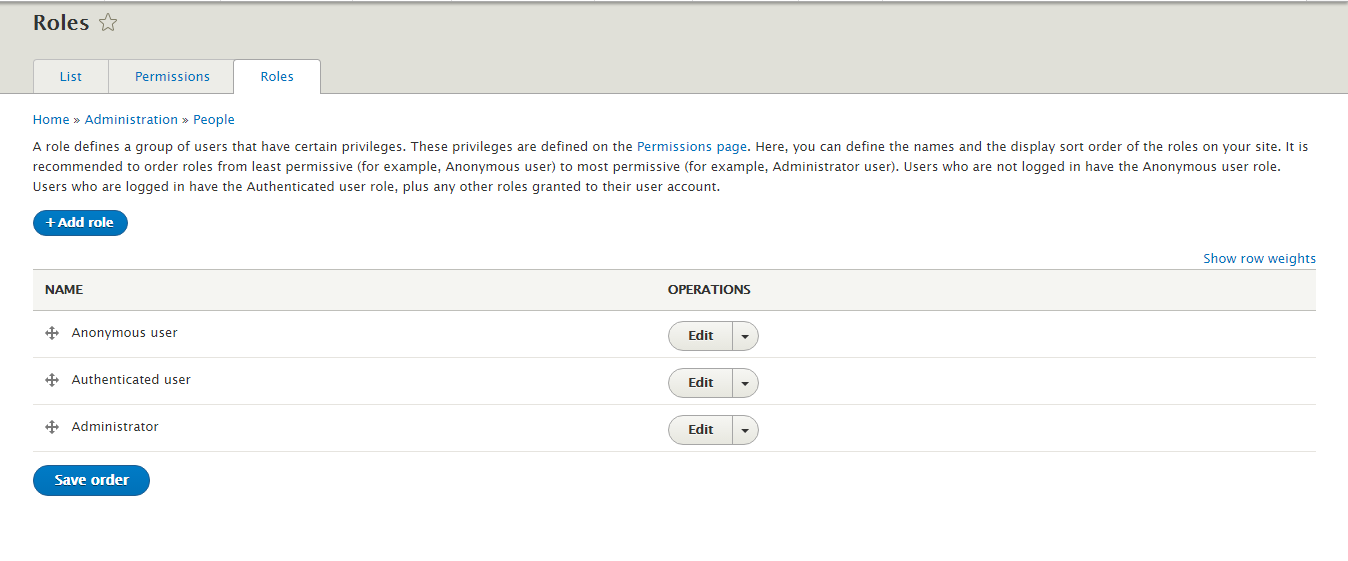
\includegraphics[width=\textwidth]{chapter6/roles_page}
   	 	\caption{Roles page.}
   	 	\label{fig:roles_page}
   	 \end{figure}
   	 
   \end{description}
   
   Next we are going to add a new role to our bitingbugs site. The role will be called \textbf{Chef}. A \textbf{Chef} can only add recipes to our site. Go to \textbf{People $\rightarrow$ Roles $\rightarrow$ Add role}. Give the new role the name \textbf{Chef} and click \textbf{Save} (Figure \ref{fig:added_chef_role}).
   
   \begin{figure}[H]
   	\centering
   	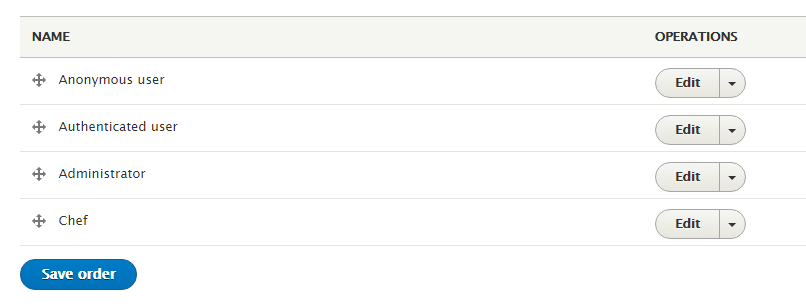
\includegraphics[width=\textwidth]{chapter6/added_chef_role}
   	\caption{Added chef role.}
   	\label{fig:added_chef_role}
   \end{figure}
   
   To change the permissions for this role go to \textbf{People $\rightarrow$ Permissions}. Under the \textbf{Chef} role check the boxes next to: \textbf{Recipe: Create new content}, \textbf{Recipe: Delete own content}, \textbf{Recipe: Edit own content} and \textbf{Use the administration toolbar} (Figure \ref{fig:edit_role_permissions}).
   
   \begin{figure}[H]
   	\centering
   	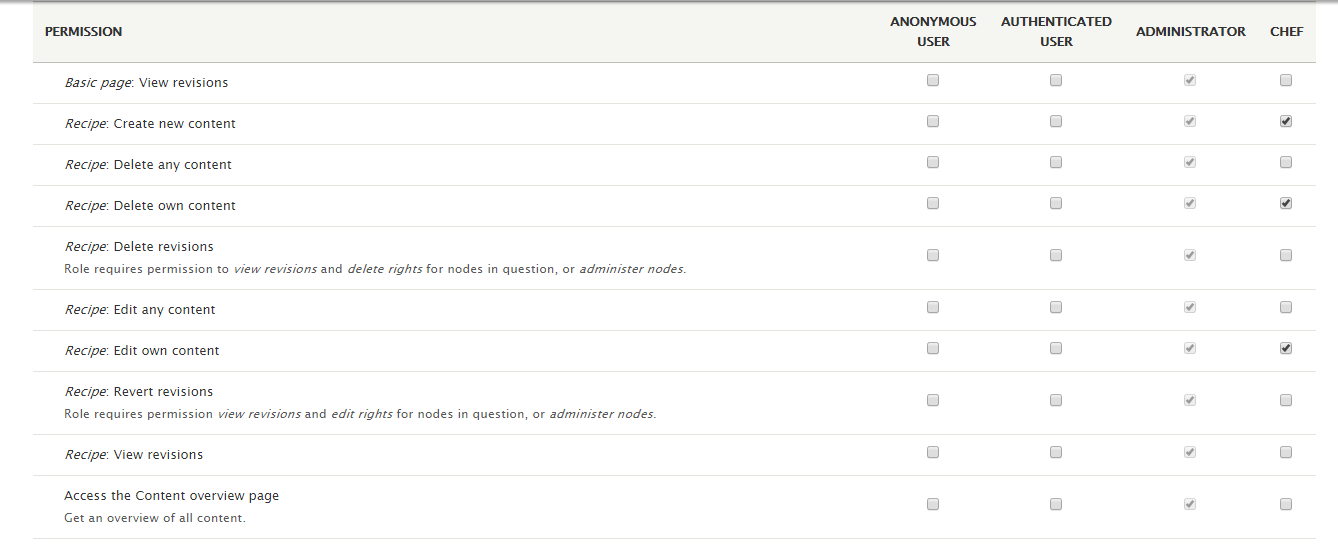
\includegraphics[width=\textwidth]{chapter6/edit_role_permissions}
   	\caption{Edit role permissions.}
   	\label{fig:edit_role_permissions}
   \end{figure}
   
   Finally we will add a new user with the role \textbf{Chef}. Go to \textbf{People $\rightarrow$ Add user}, enter the following information:
   
   \begin{description}
   	\item[Email address:] chefjohn@bitingbugs.be
   	\item[Username:] Chefjohn
   	\item[Password:] ICanCook
   	\item[Status:] Active
   	\item[Roles:] \textbf{Authenticated user} and \textbf{Chef}
   	\item[Picture:] \textbf{chapter6/chefjohn.jpg}
   	\item[Site language:] English
   	\item[Contact settings:] Personal contact form
   	\item[Time zone:] Europe/Brussels
   \end{description}
   
   Click the \textbf{Create new account} button. By default Drupal redirects back to the \textbf{Create new account} page because you usually want to add multiple users. We will not add any more users for now. Go back to the \textbf{People} page, there you can see the new user we added. 
   When we login with the chefjohn account we see the following menu:  
   
   \begin{figure}[H]
   	\centering
   	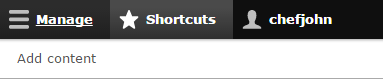
\includegraphics[width=\textwidth]{chapter6/chef_menu}
   	\caption{The menu for the \textbf{Chef} role.}
   	\label{fig:chef_menu}
   \end{figure}
   
   As you can see a \textbf{Chef} can only add recipes.
   
   \section{Views}
   
   \subsection{Settings}
   
   Views is a query builder. It basically builds lists of content, and displays them in any format
   we choose. Views comes with a few standard preconfigured lists, e.g. a list to replace the
   standard front page, a list of recent comments, etc\ldots
   
   Views has a few settings that we like to turn on. On the \textbf{Structure $\rightarrow$ Views} page, click the
   \textbf{Settings} tab.
   
   \begin{figure}[H]
   	\centering
   	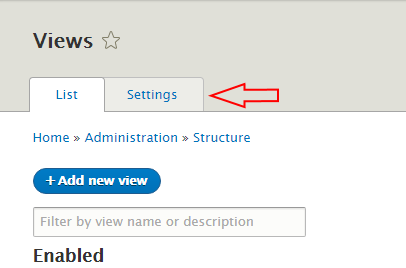
\includegraphics[width=\textwidth]{chapter6/views_settings}
   	\label{fig:views_settings}
   \end{figure}
   
   This will take you to the following page.
   
   \begin{figure}[H]
   	\centering
   	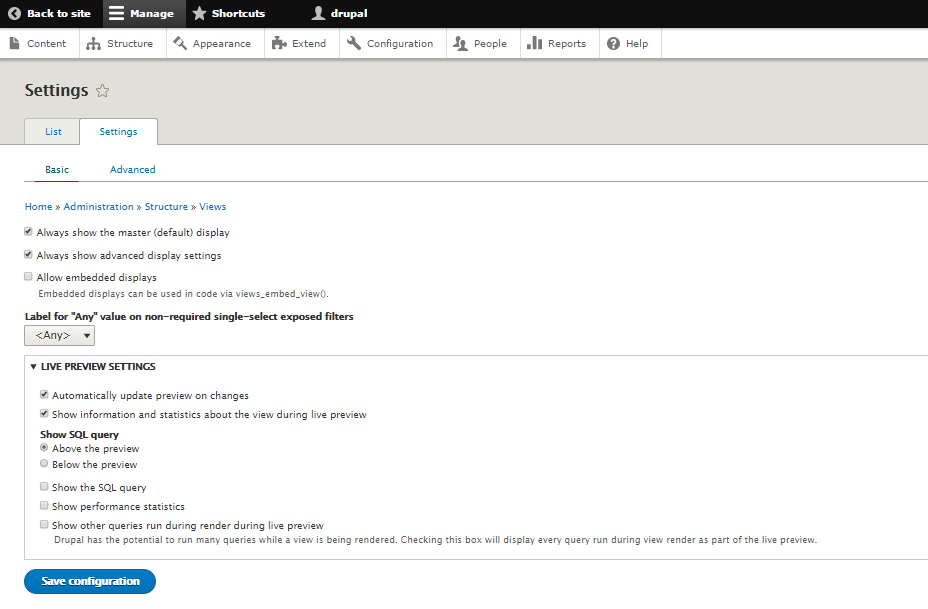
\includegraphics[width=\textwidth]{chapter6/views_settings_page}
   	\caption{The views settings page.}
   	\label{fig:views_settings_page}
   \end{figure}
   
   Enable the \textbf{Always show the master display} and \textbf{Always show advanced display settings} settings.
   
   Also enable the \textbf{Automatically update preview on changes} setting. 
   
   The \textbf{Show information and statistics} option and the \textbf{SQL query options} are useful when there
   is a problem and you are debugging what is wrong, you can turn this on as well.
   
   \subsection{Creating a view}
   
   To create a new view go to \textbf{Structure $\rightarrow$ Views $\rightarrow$ Add new view}. 
   
   Now you can provide a View name, and choose what you want to display (content,
   taxonomy, files, users\ldots).
   
   Besides that, you can also choose one or two displays to start with. If you want your view to
   be displayed as a page, select the \textbf{Create a page} option. You will have to provide a Page title
   and Path. All these settings can be altered afterwards.
   
   You can also choose to display the view in a block by selecting Create a block. In this case you will need to give it a \textbf{Block title}. When you are done, click \textbf{Save and edit} (Figure \ref{fig:new_view_settings}).
   
   
   
   
   
   
   \section{Review exercises}
   
   \begin{enumerate}
    \item Add a new role \textbf{Content manager}. A content manager can create, delete and edit all content but nothing else.
    \item Create a new content manager named \textbf{managerpaul}.
   \end{enumerate}
   